\documentclass[12pt]{article}
\usepackage{tikz}
\usepackage[cm]{fullpage}
\usepackage{verbatim}
\usepackage{hyperref} 
\usepackage{graphicx}
\usepackage{natbib}
\usepackage{amsmath,amssymb}
\usetikzlibrary{arrows}
\usepackage{dsfont}
\DeclareMathOperator*{\argmin}{arg\,min}
\DeclareMathOperator*{\sign}{sign}
\DeclareMathOperator*{\Lik}{Lik}
\DeclareMathOperator*{\Peaks}{Peaks}
\DeclareMathOperator*{\HotSpots}{HotSpots}
\newcommand{\Cost}{\text{Cost}}
\DeclareMathOperator*{\Diag}{Diag}
\DeclareMathOperator*{\TPR}{TPR}
\DeclareMathOperator*{\FPR}{FPR}
\DeclareMathOperator*{\argmax}{arg\,max}
\DeclareMathOperator*{\maximize}{maximize}
\DeclareMathOperator*{\minimize}{minimize}
\newcommand{\ZZ}{\mathbb Z}
\newcommand{\NN}{\mathbb N}
\newcommand{\RR}{\mathbb R}
\newtheorem{definition}{Definition}

\begin{document}

\title{Constrained maximum likelihood binomial segmentation model for
  changepoint detection in methylation count data}

\author{Toby Dylan Hocking}

\maketitle

\section{Introduction/problem}

We use the notation of \citet{smoothedEM}. For each site $i\in\{1,\dots, N\}$ let 
\begin{itemize}
\item $X_i\in\ZZ_+$ be the total observed count of combined C reads and T reads,
\item $Y_i\in\ZZ_+$ be the observed count of C reads,
\item $S_i\in\{0,1\}$ be the unobserved methylation status (1=unmethylated, 0=methylated),
\item $P_i\in[0,1]$ be the unobserved proportion of methylated reads
  (the segment mean, which we will constrain to have a few distinct changepoints).
\end{itemize}

\section{Statistical model and loss function}

Our model is $Y_i \sim \text{Binomial}(X_i, P_i)$. Maximizing the
log-likelihood is equivalent to minimizing this loss function:
\begin{equation}
  \label{eq:binomial_loss}
  \ell_i(p) = (Y_i - X_i) \log(1-p) - Y_i\log p
\end{equation}

\subsection{State-based changepoint model}

We propose to
solve the following optimal changepoint detection problem. Let
$G=(V,E)$ be a directed graph that represents the model
states/changes/constraints (Figure~\ref{fig:state-graphs}). There are two
vertices $V=\{0=\text{methylated},1=\text{unmethylated}\}$, one for
each of the two states. There are two edges
$E=\{1,-1\}$, one for each possible change between
states. Each edge/change $c\in E$ has corresponding data
$(\underline v_c, \overline v_c, \lambda_c, g_c)$ which specifies a
transition from state $\underline v_c$ to state $\overline v_c$, with
a penalty of $\lambda_c\in\RR_+$, and a constraint function
$g_c:\RR\times\RR\rightarrow\RR$ (for our model these values are given
in Table~\ref{tab:changes}).
\begin{table}
  \centering
\begin{tabular}{cllcl}
change $c$ &  from $\underline v_c$ & to $\underline v_c$ & penalty $\lambda_c$ & constraint $g_c$ \\
\hline
-1 & $S=0$ methylated & $S=1$ unmethylated & $\lambda_\downarrow$ & non-increasing $g_\downarrow$\\
1 &$S=1$ unmethylated & $S=0$ methylated & $\lambda_\uparrow$ & non-decreasing $g_\uparrow$
\end{tabular}
\caption{Changes possible in our model. Note that typically we would take $\lambda_\uparrow=\lambda_\downarrow$ 
  so that non-increasing and non-decreasing changes are equally penalized.}
  \label{tab:changes}
\end{table}
\begin{figure*}
\centering
  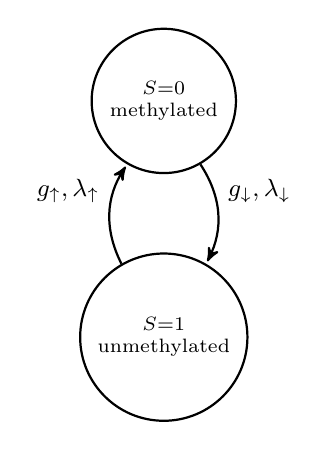
\begin{tikzpicture}[->,>=stealth',shorten >=1pt,auto,node distance=3cm,
                    thick,main node/.style={circle,draw}]

  \node[main node] (1) {$S=0 \atop \text{methylated}$ };
  \node[main node] (2) [below of=1] {$S=1\atop \text{unmethylated}$ };

  \path[every node/.style={font=\sffamily\small}]
    (2) edge [bend left] node {$g_\uparrow, \lambda_\uparrow$} (1)
    (1) edge [bend left] node {$g_\downarrow, \lambda_\downarrow$} (2);
\end{tikzpicture}
\caption{State/change graph for our model. Nodes represent
  states $S_i$ and edges represent changes $c_i$. Each change has a corresponding
  penalty $\lambda$, and a function $g$ that determines what types of
  changes are possible ($g_\uparrow$ non-decreasing,
  $g_\downarrow$ non-increasing). Even though there are no edges from a node
  to itself, it is still possible to stay in the same state without
  introducing a changepoint and penalty. }
  \label{fig:state-graphs}
\end{figure*}

\subsection{Optimization problem}

The optimization problem below searches for the best mean/proportion
$\mathbf p$, changepoints $\mathbf c$, and states $\mathbf s$. Note
that for the changepoint variables we allow $c_i=0$, which implies no
penalty $\lambda_0=0$, and means no change:
\begin{align}
  \label{eq:GFPOP_problem}
  \minimize_{
    \substack{
    \mathbf p\in\RR^N,\ \mathbf s\in \{0,1\}^N\\
\mathbf c\in \{-1,0,1\}^{N-1}
}
    } &\ \ 
  \sum_{i=1}^N \ell_i(p_i) + \sum_{i=1}^{N-1} \lambda_{c_i} \\
  \text{subject to \hskip 0.9cm} &\ \ c_i = 0 \Rightarrow p_i = p_{i+1}
\text{ and } s_i = s_{i+1},
\label{eq:no_change}\\
\label{eq:change_non_dec}&\ \ c_i =1 \Rightarrow p_i \leq p_{i+1} \text{ and } s_i=1,\ s_{i+1}=0,
\\
\label{eq:change_non_inc}&\ \ c_i =-1 \Rightarrow p_i \geq p_{i+1} \text{ and } s_i=0,\ s_{i+1}=1.
\end{align}

The constraints are interpreted as follows:
\begin{itemize}
\item (\ref{eq:no_change}) $c_i=0$ means no change between data points $i$ and $i+1$, 
\item (\ref{eq:change_non_inc}) $c_i=-1$ means a non-increasing change,
\item (\ref{eq:change_non_dec}) $c_i=1$ means a non-decreasing change.
\end{itemize}

If some states are desired at the start or end, then those constraints
$s_1\in \underline S, s_n\in\overline S$ can also be enforced. (those
kind of constraints are useful in ChIP-seq because we know there are
no peaks in the start/end of the chromosome, but I don't think they
are useful in methylation data -- do we know in advance if the
start/end of the chromosome should be methylated?)

\subsection{Dynamic programming update rules}  To compute the
solution to optimization problem (\ref{eq:GFPOP_problem}), we propose the following
dynamic programming algorithm.

\begin{figure}
\centering
  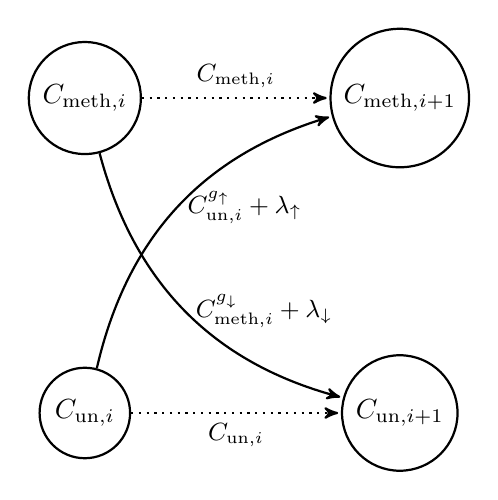
\begin{tikzpicture}[->,>=stealth',shorten >=1pt,auto,node distance=4cm,
  thick,main node/.style={circle,draw}]
  \node[main node] (peak_t) {$C_{\text{meth},i}$};
  \node[main node] (bkg_t) [below of=peak_t] {$C_{\text{un}, i}$};
  \node[main node] (peak_t1) [right of=peak_t] {$C_{\text{meth}, i+1}$};
  \node[main node] (bkg_t1) [right of=bkg_t] {$C_{\text{un}, i+1}$};
  \path[every node/.style={font=\small}]
    (peak_t) edge [dotted] node {$C_{\text{meth}, i}$} (peak_t1)
    (peak_t) edge [black, bend right] node [right] {$C_{\text{meth}, i}^{g_\downarrow}+\lambda_\downarrow$} (bkg_t1)
    (bkg_t) edge [dotted] node[midway, below] {$C_{\text{un}, i}$} (bkg_t1)
    (bkg_t) edge [black, bend left] node[right] {$C_{\text{un}, i}^{g_\uparrow}+\lambda_\uparrow$} (peak_t1)
;
\end{tikzpicture}
\caption{Computation graph which represents the dynamic programming
  updates (\ref{eq:C_meth},\ref{eq:C_un}) for the state graph model in
  Figure~\ref{fig:state-graphs}. Nodes represent cost functions
  $C_{s,i}$ in each state $s$ at data $i$ and $i+1$. Edges represent
  inputs to the $\min\{\}$ operation (solid for a changepoint, dotted
  for no change). $S=0$ methylated state is abbreviated as ``meth'' and $S=1$ unmethylated state is abbreviated as ``un''.}
  \label{fig:computation-graphs}
\end{figure}

Let $C_{s,i}(p)$ be the optimal cost with mean/proportion $p$ and
state $s$ at data point $i$. This quantity can be recursively computed
using dynamic programming. The initialization for the first data point
is $ C_{s,1}(p) = \ell_i(p)$ for both states
$s\in\{\text{meth}=0,\text{un}=1\}$. The dynamic programming update
rule to compute the best cost up to data points $i>1$, if data point
$i$ is methylated, is
\begin{equation}
\label{eq:C_meth}
   C_{\text{meth},i}(p) = \ell_i(p) + \min\{
  C_{\text{meth},i-1}(p)
  ,\,
  C^\leq_{\text{un},i-1}(p) + \lambda_\uparrow
  \},
\end{equation}
where the min-less operator $C^\leq$ is defined as below. (this
definition follows from the fact that we want to constrain a
non-decreasing change, for details read \citet{HockingGFPOP})
\begin{definition}[Min-less operator]
\label{def:min-less}
  Given any real-valued function $f:\RR\rightarrow\RR$, we define its min-less
  operator as $f^\leq(\mu)=\min_{x\leq \mu} f(x)$.
\end{definition}
Intuitively, the best cost (\ref{eq:C_meth}) is equal to the min of two possible costs: 
\begin{itemize}
\item the first option $C_{\text{meth},i-1}(p)$ is if there is no
  change from the previous data point $i-1$ which was also methylated,
\item the second option $C^\leq_{\text{un},i-1}(p) + \lambda_\uparrow$
  is if there is a non-decreasing change from an unmethylated state at
  the previous data point $i-1$.
\end{itemize}
The dynamic programming update for the best unmethylated cost is analogous:
\begin{equation}
\label{eq:C_un}
   C_{\text{un},i}(p) = \ell_i(p) + \min\{
  C_{\text{un},i-1}(p)
  ,\,
  C^\geq_{\text{meth},i-1}(p) + \lambda_\downarrow
  \}.
\end{equation}
where the min-more operator $C^\geq$ is defined as below.
\begin{definition}[Min-more operator]
\label{def:min-more}
  Given any real-valued function $f:\RR\rightarrow\RR$, we define its min-more
  operator as $f^\geq(\mu)=\min_{x\geq \mu} f(x)$.
\end{definition}

The computations required for the dynamic programming updates
(\ref{eq:C_meth},\ref{eq:C_un}) can be visualized using a computation graph
(Figure~\ref{fig:computation-graphs}).

Note that these update rules are guaranteed to compute the optimal
solution to this non-convex problem (\ref{eq:GFPOP_problem}).
 
\subsection{Root finding}

To perform the dynamic programming updates for the binomial
distribution we need to be able to find the solution of
\begin{equation}
  \label{eq:pDPA-intervals}
  a \log(1-p) + b \log p + c = d
\end{equation}
in terms of $p$, where $a,b,c,d$ are constants which depend on the
data. From experience implementing a root finder for the Poisson loss,
it will be advantageous (faster convergence) to do the root finding in
another space, where the tails are linear.

Let $u=\log p - \log(1-p) = \log(\frac{p}{1-p})\in\RR$ be that new
variable, so $p=(1+e^{-u})^{-1}$. Thus
\begin{eqnarray*}
  \ell_i(p) 
  &=& (m_i - t_i) \log(1-p) - m_i\log p \\
  &=& (m_i - t_i) \log(1-\frac{1}{1+e^{-u}}) - m_i\log(\frac{1}{1+e^{-u}})\\
g_i(u)  &=& (t_i - m_i) \log(e^u+1) + m_i\log(1+e^{-u}) \\
\end{eqnarray*}
The equation above can be used to update/add the cost of a new data
point. We will thus need to store and find roots of functions such as
the one below, 
\begin{equation}
  \label{eq:g(u)}
  g(u)=a\log(1+e^u)+b\log(1+e^{-u})+c=d,
\end{equation}
where we will store the coefficients $a,b,c$ as double
precision floating point numbers. The derivatives are
\begin{equation}
  \label{eq:g'(u)}
  g'(u)=\frac{ae^u - b}{1+e^u} = \frac{a-be^{-u}}{e^{-u}+1}.
\end{equation}
The equations above make it clear that the asymptotes are linear. As
$u\rightarrow\infty$, $g'(u)\rightarrow a$. As $u\rightarrow -\infty$,
$g'(u)\rightarrow -b$. They also can be used to show that the minimum
of the loss function occurs at $u=\log(b/a)$.  Depending on whether we
are looking for the smaller or larger root, we can start the root
finding on one side or the other of the minimum:
$u_0 = \log(b/a)\pm 1$. Then the updates are for each iteration $i>0$,
$u_i = u_{i-1} - g(u_{i-1})/g'(u_{i-1})$. We can stop the root when
the cost is below some small absolute value, such as $10^{-12}$. For
large data we should store the mean cost rather than the total cost,
for numerical stability.

\subsection{On-disk implementation for large data}

For really large genomic data ($N>10^6$) we will need to store the
$O(N)$ cost functions $C_i(p)$ on disk, to avoid memory problems. We
can use BerkeleyDB STL as in
PeakSegPipeline::PeakSegFPOP\_disk\footnote{\url{https://github.com/tdhock/PeakSegPipeline/blob/master/src/PeakSegFPOPLog.cpp}}.

\bibliographystyle{abbrvnat}

\bibliography{refs}

\end{document}
